% Generated by draw_lafont.py.
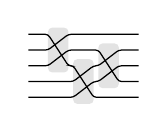
\begin{tikzpicture}[x=1cm,y=1cm,baseline={([yshift=-0.25em]mid)},line width=.45pt]
\coordinate (mid) at (0,-0.400);
\fill[black!11,rounded corners=1.5pt] (0.250,-0.484) rectangle (0.510,0.084);
\fill[black!11,rounded corners=1.5pt] (0.570,-0.884) rectangle (0.830,-0.316);
\fill[black!11,rounded corners=1.5pt] (0.890,-0.684) rectangle (1.150,-0.116);
\draw[rounded corners=1pt] (0.000,-0.800)--(0.570,-0.800)--(0.830,-0.600)--(0.890,-0.600)--(1.150,-0.400)--(1.400,-0.400);
\draw[rounded corners=1pt] (0.000,-0.600)--(0.570,-0.600)--(0.830,-0.400)--(0.890,-0.400)--(1.150,-0.200)--(1.400,-0.200);
\draw[rounded corners=1pt] (0.000,-0.400)--(0.250,-0.400)--(0.510,-0.200)--(0.890,-0.200)--(1.150,-0.600)--(1.400,-0.600);
\draw[rounded corners=1pt] (0.000,-0.200)--(0.250,-0.200)--(0.510,0.000)--(1.400,0.000);
\draw[rounded corners=1pt] (0.000,0.000)--(0.250,0.000)--(0.510,-0.400)--(0.570,-0.400)--(0.830,-0.800)--(1.400,-0.800);
\end{tikzpicture}
